\problemname{Astronomer}
\illustration{.3}{img/TychoBrahe.JPG}{}

\noindent
The astronomer has a passion for stargazing.
In particular, he gets immense pleasure out of gazing at $k$~stars simultaneously through his telescope.   
Building a telescope with radius~$r$ costs $t\cdot r$~kroner.
A newly built telescope will point exactly at the origin $(0,0)$.
Moving it to point somewhere else also takes effort; 
shifting the telescope a distance of $d$~units incurs a cost of $s\cdot d$~kroner.
The astronomer can observe all stars at distance at most $r$ from where the telescope points.

How much does it cost to build and move a telescope that allows $k$~stars to be observed at once?

\medskip

All coordinates and distances are given in the Euclidean plane.


\section*{Example}

Here is an example with $n=3$ stars at positions $(0,0)$, $(2,0)$, and $(3,1)$.
The shaded area shows a telescope of radius~$1$ pointing at $(1,0)$ covering two stars; this costs $s + t$~kroner and is an optimal solution to sample input~$3$.
The image also shows optimal solutions to sample inputs~$1$, $2$, and $4$.

\medskip
\noindent
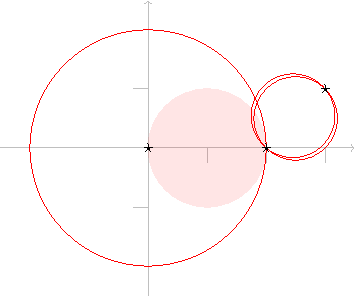
\includegraphics[width=.3\textwidth]{img/samples.pdf}


\section*{Input}

The first line consists of four integers:
the number~$k$ of stars the astronomer wants to observe,
the number~$n$ of stars in tonight's sky,
the shifting cost~$s$, and
the telescope building cost~$t$.
Then follow $n$ lines, where the $i$th line contains the integer coordinates $x_i$ and $y_i$ of the $i$th star.

\section*{Output}

A single real number: the minimum number of kroner that the astronomer needs to spend.

\section*{Constraints and Scoring}

You can assume 
\begin{enumerate}
\item $1\leq k\leq n\leq 700$. % constraint:kn
\item $x_i, y_i\in \{-10^9,\ldots, 10^9\}$ for all $i\in\{1,\ldots,n\}$. % constraint:xy
\item $s,t\in \{0,\ldots, 10^9\}$. % constraint:st
\item Your output is accepted if it is within a relative or absolute tolerance of $\epsilon = 10^{-6}$ of the correct answer.
\end{enumerate}


Your solution will be tested on a set of test groups, each worth a number of points.
Each test group contains a set of test cases.
To get the points for a test group you need to solve all test cases in the test group.
Your final score will be the maximum score of a single submission.

\medskip
\noindent
\begin{tabular}{lll}
  Group & Points & Constraints\\\hline
  $1$ & $8$ &  $t\leq s$\\
  $2$ & $9$ & $n\le 50$ and $s=0$\\
  $3$ & $18$ & $s=0$\\
  $4$ & $13$ & $n\leq 50$\\
  $5$ & $14$ & $n\leq 350$\\
  $6$ & $15$ & $\epsilon = 1/10$\\
  $7$ & $23$ & \emph{No further constraints}\\
\end{tabular}
